\documentclass{standalone}
\usepackage{tikz}
\usetikzlibrary{patterns, positioning}


\begin{document}
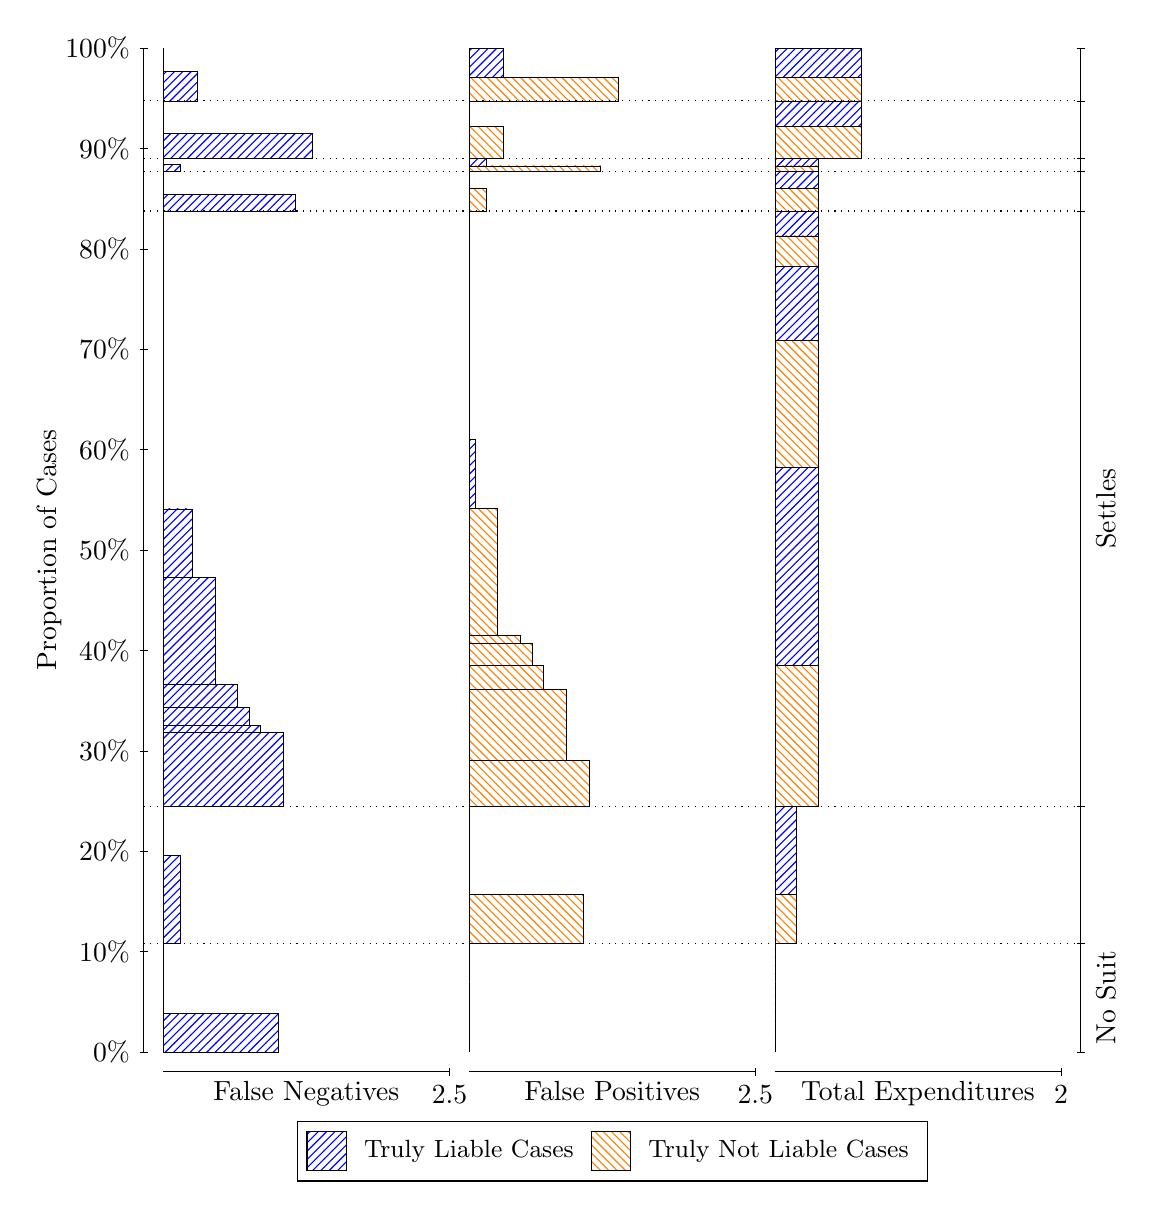
\begin{tikzpicture}
\draw[black, very thin] (1.5,1.75) -- (1.5,14.5);
\node[rotate=90, text=black, anchor=center] at (0.3, 8.125) {Proportion of Cases};
\draw[black, very thin] (1.45,1.75) -- (1.55,1.75);
\node[text=black, anchor=east] at (1.45, 1.75) {0\%};
\draw[black, very thin] (1.45,3.025) -- (1.55,3.025);
\node[text=black, anchor=east] at (1.45, 3.025) {10\%};
\draw[black, very thin] (1.45,4.3) -- (1.55,4.3);
\node[text=black, anchor=east] at (1.45, 4.3) {20\%};
\draw[black, very thin] (1.45,5.575) -- (1.55,5.575);
\node[text=black, anchor=east] at (1.45, 5.575) {30\%};
\draw[black, very thin] (1.45,6.85) -- (1.55,6.85);
\node[text=black, anchor=east] at (1.45, 6.85) {40\%};
\draw[black, very thin] (1.45,8.125) -- (1.55,8.125);
\node[text=black, anchor=east] at (1.45, 8.125) {50\%};
\draw[black, very thin] (1.45,9.4) -- (1.55,9.4);
\node[text=black, anchor=east] at (1.45, 9.4) {60\%};
\draw[black, very thin] (1.45,10.675) -- (1.55,10.675);
\node[text=black, anchor=east] at (1.45, 10.675) {70\%};
\draw[black, very thin] (1.45,11.95) -- (1.55,11.95);
\node[text=black, anchor=east] at (1.45, 11.95) {80\%};
\draw[black, very thin] (1.45,13.225) -- (1.55,13.225);
\node[text=black, anchor=east] at (1.45, 13.225) {90\%};
\draw[black, very thin] (1.45,14.5) -- (1.55,14.5);
\node[text=black, anchor=east] at (1.45, 14.5) {100\%};

\draw[black, very thin] (13.4,1.75) -- (13.4,14.5);
\draw[black, very thin] (13.35,1.75) -- (13.45,1.75);
\node[anchor=west] at (13.35, 1.75) {};
\draw[black, very thin] (13.35,3.1277) -- (13.45,3.1277);
\node[anchor=west] at (13.35, 3.1277) {};
\draw[black, very thin] (13.35,4.8723) -- (13.45,4.8723);
\node[anchor=west] at (13.35, 4.8723) {};
\draw[black, very thin] (13.35,12.43) -- (13.45,12.43);
\node[anchor=west] at (13.35, 12.43) {};
\draw[black, very thin] (13.35,12.931) -- (13.45,12.931);
\node[anchor=west] at (13.35, 12.931) {};
\draw[black, very thin] (13.35,13.095) -- (13.45,13.095);
\node[anchor=west] at (13.35, 13.095) {};
\draw[black, very thin] (13.35,13.83) -- (13.45,13.83);
\node[anchor=west] at (13.35, 13.83) {};
\draw[black, very thin] (13.35,14.5) -- (13.45,14.5);
\node[anchor=west] at (13.35, 14.5) {};

\draw[black, very thin, pattern color=blue, pattern=north east lines] (1.75,1.75) rectangle (3.2033,2.2355);
\draw[black, very thin, pattern color=orange, pattern=north west lines] (1.75,2.2355) rectangle (1.75,3.1277);
\draw[black, very thin, pattern color=blue, pattern=north east lines] (1.75,3.1277) rectangle (1.968,4.2445);
\draw[black, very thin, pattern color=orange, pattern=north west lines] (1.75,4.2445) rectangle (1.75,4.8723);
\draw[black, very thin, pattern color=blue, pattern=north east lines] (1.75,4.8723) rectangle (3.276,5.8104);
\draw[black, very thin, pattern color=blue, pattern=north east lines] (1.75,5.8104) rectangle (2.9853,5.8937);
\draw[black, very thin, pattern color=blue, pattern=north east lines] (1.75,5.8937) rectangle (2.84,6.1259);
\draw[black, very thin, pattern color=blue, pattern=north east lines] (1.75,6.1259) rectangle (2.6947,6.4146);
\draw[black, very thin, pattern color=blue, pattern=north east lines] (1.75,6.4146) rectangle (2.404,7.7759);
\draw[black, very thin, pattern color=blue, pattern=north east lines] (1.75,7.7759) rectangle (2.1133,8.647);
\draw[black, very thin, pattern color=orange, pattern=north west lines] (1.75,8.647) rectangle (1.75,12.43);
\draw[black, very thin, pattern color=blue, pattern=north east lines] (1.75,12.43) rectangle (3.4213,12.643);
\draw[black, very thin, pattern color=orange, pattern=north west lines] (1.75,12.643) rectangle (1.75,12.931);
\draw[black, very thin, pattern color=blue, pattern=north east lines] (1.75,12.931) rectangle (1.968,13.025);
\draw[black, very thin, pattern color=orange, pattern=north west lines] (1.75,13.025) rectangle (1.75,13.095);
\draw[black, very thin, pattern color=blue, pattern=north east lines] (1.75,13.095) rectangle (3.6393,13.418);
\draw[black, very thin, pattern color=orange, pattern=north west lines] (1.75,13.418) rectangle (1.75,13.83);
\draw[black, very thin, pattern color=blue, pattern=north east lines] (1.75,13.83) rectangle (2.186,14.199);
\draw[black, very thin, pattern color=orange, pattern=north west lines] (1.75,14.199) rectangle (1.75,14.5);
\draw[black, very thin, pattern color=orange, pattern=north west lines] (5.6333,1.75) rectangle (5.6333,2.6422);
\draw[black, very thin, pattern color=blue, pattern=north east lines] (5.6333,2.6422) rectangle (5.6333,3.1277);
\draw[black, very thin, pattern color=orange, pattern=north west lines] (5.6333,3.1277) rectangle (7.0867,3.7555);
\draw[black, very thin, pattern color=blue, pattern=north east lines] (5.6333,3.7555) rectangle (5.6333,4.8723);
\draw[black, very thin, pattern color=orange, pattern=north west lines] (5.6333,4.8723) rectangle (7.1593,5.4484);
\draw[black, very thin, pattern color=orange, pattern=north west lines] (5.6333,5.4484) rectangle (6.8687,6.3524);
\draw[black, very thin, pattern color=orange, pattern=north west lines] (5.6333,6.3524) rectangle (6.578,6.6562);
\draw[black, very thin, pattern color=orange, pattern=north west lines] (5.6333,6.6562) rectangle (6.4327,6.9398);
\draw[black, very thin, pattern color=orange, pattern=north west lines] (5.6333,6.9398) rectangle (6.2873,7.0449);
\draw[black, very thin, pattern color=orange, pattern=north west lines] (5.6333,7.0449) rectangle (5.9967,8.6554);
\draw[black, very thin, pattern color=blue, pattern=north east lines] (5.6333,8.6554) rectangle (5.706,9.5265);
\draw[black, very thin, pattern color=blue, pattern=north east lines] (5.6333,9.5265) rectangle (5.6333,12.43);
\draw[black, very thin, pattern color=orange, pattern=north west lines] (5.6333,12.43) rectangle (5.8513,12.718);
\draw[black, very thin, pattern color=blue, pattern=north east lines] (5.6333,12.718) rectangle (5.6333,12.931);
\draw[black, very thin, pattern color=orange, pattern=north west lines] (5.6333,12.931) rectangle (7.3047,13.002);
\draw[black, very thin, pattern color=blue, pattern=north east lines] (5.6333,13.002) rectangle (5.8513,13.095);
\draw[black, very thin, pattern color=orange, pattern=north west lines] (5.6333,13.095) rectangle (6.0693,13.508);
\draw[black, very thin, pattern color=blue, pattern=north east lines] (5.6333,13.508) rectangle (5.6333,13.83);
\draw[black, very thin, pattern color=orange, pattern=north west lines] (5.6333,13.83) rectangle (7.5227,14.131);
\draw[black, very thin, pattern color=blue, pattern=north east lines] (5.6333,14.131) rectangle (6.0693,14.5);
\draw[black, very thin, pattern color=orange, pattern=north west lines] (9.5167,1.75) rectangle (9.5167,2.6422);
\draw[black, very thin, pattern color=blue, pattern=north east lines] (9.5167,2.6422) rectangle (9.5167,3.1277);
\draw[black, very thin, pattern color=orange, pattern=north west lines] (9.5167,3.1277) rectangle (9.7892,3.7555);
\draw[black, very thin, pattern color=blue, pattern=north east lines] (9.5167,3.7555) rectangle (9.7892,4.8723);
\draw[black, very thin, pattern color=orange, pattern=north west lines] (9.5167,4.8723) rectangle (10.062,6.6562);
\draw[black, very thin, pattern color=blue, pattern=north east lines] (9.5167,6.6562) rectangle (10.062,9.1773);
\draw[black, very thin, pattern color=orange, pattern=north west lines] (9.5167,9.1773) rectangle (10.062,10.788);
\draw[black, very thin, pattern color=blue, pattern=north east lines] (9.5167,10.788) rectangle (10.062,11.726);
\draw[black, very thin, pattern color=orange, pattern=north west lines] (9.5167,11.726) rectangle (10.062,12.115);
\draw[black, very thin, pattern color=blue, pattern=north east lines] (9.5167,12.115) rectangle (10.062,12.43);
\draw[black, very thin, pattern color=orange, pattern=north west lines] (9.5167,12.43) rectangle (10.062,12.718);
\draw[black, very thin, pattern color=blue, pattern=north east lines] (9.5167,12.718) rectangle (10.062,12.931);
\draw[black, very thin, pattern color=orange, pattern=north west lines] (9.5167,12.931) rectangle (10.062,13.002);
\draw[black, very thin, pattern color=blue, pattern=north east lines] (9.5167,13.002) rectangle (10.062,13.095);
\draw[black, very thin, pattern color=orange, pattern=north west lines] (9.5167,13.095) rectangle (10.607,13.508);
\draw[black, very thin, pattern color=blue, pattern=north east lines] (9.5167,13.508) rectangle (10.607,13.83);
\draw[black, very thin, pattern color=orange, pattern=north west lines] (9.5167,13.83) rectangle (10.607,14.131);
\draw[black, very thin, pattern color=blue, pattern=north east lines] (9.5167,14.131) rectangle (10.607,14.5);
\draw[black, dotted] (1.5,3.1277) -- (13.4,3.1277);
\draw[black, dotted] (1.5,4.8723) -- (13.4,4.8723);
\draw[black, dotted] (1.5,12.43) -- (13.4,12.43);
\draw[black, dotted] (1.5,12.931) -- (13.4,12.931);
\draw[black, dotted] (1.5,13.095) -- (13.4,13.095);
\draw[black, dotted] (1.5,13.83) -- (13.4,13.83);
\draw[black, very thin] (1.75,1.5) -- (5.3833,1.5);
\node[text=black, anchor=north] at (3.5667, 1.5) {False Negatives};
\draw[black, very thin] (5.3833,1.45) -- (5.3833,1.55);
\node[text=black, anchor=north] at (5.3833, 1.45) {2.5};

\draw[black, very thin] (5.6333,1.5) -- (9.2667,1.5);
\node[text=black, anchor=north] at (7.45, 1.5) {False Positives};
\draw[black, very thin] (9.2667,1.45) -- (9.2667,1.55);
\node[text=black, anchor=north] at (9.2667, 1.45) {2.5};

\draw[black, very thin] (9.5167,1.5) -- (13.15,1.5);
\node[text=black, anchor=north] at (11.333, 1.5) {Total Expenditures};
\draw[black, very thin] (13.15,1.45) -- (13.15,1.55);
\node[text=black, anchor=north] at (13.15, 1.45) {2};

\node[text=black, centered, rotate=90] at (13.72, 2.4389) {No Suit};

\node[text=black, centered, rotate=90] at (13.72, 8.6512) {Settles};





\draw (7.449999999999999,1.5) node[draw=none] (baseCoordinate) {};
\begin{scope}[align=center]
        \matrix[scale=0.5, draw=black, below=0.5cm of baseCoordinate, nodes={draw}, column sep=0.1cm]{
            \node[rectangle, draw, minimum width=0.5cm, minimum height=0.5cm, pattern color=blue, pattern=north east lines] {}; &
            \node[draw=none, font=\small, text=black] (B) {Truly Liable Cases}; &
            \node[rectangle, draw, minimum width=0.5cm, minimum height=0.5cm, pattern color=orange, pattern=north west lines] {}; &
            \node[draw=none, font=\small, text=black] (B) {Truly Not Liable Cases}; \\
            };
\end{scope}

\end{tikzpicture}
\end{document}